\documentclass[a4paper,14pt]{extreport} %размер бумаги устанавливаем А4, шрифт 12пунктов
\renewcommand{\rmdefault}{ftm}
\renewcommand{\baselinestretch}{1.5}
\newcommand{\mychapter}[1]{\chapter*{#1} \addcontentsline{toc}{chapter}{#1} \refstepcounter{chapter}}\usepackage[T2A]{fontenc}
\usepackage[utf8]{inputenc}%включаем кодировку utf8
\usepackage[english,russian]{babel}%используем русский и английский языки с переносами
\usepackage{amssymb,amsfonts,amsmath,mathtext,cite,enumerate,float} %подключаем нужные пакеты расширений
\usepackage{graphicx} %хотим вставлять в диплом рисунки?
\graphicspath{{fig/intro/}}%путь к рисункам
\makeatletter
\renewcommand{\@biblabel}[1]{#1.} % Заменяем библиографию с квадратных скобок на точку:
\makeatother

\usepackage{geometry} % Меняем поля страницы
\geometry{left=2.5cm}% левое поле
\geometry{right=1cm}% правое поле
\geometry{top=2cm}% верхнее поле
\geometry{bottom=2.5cm}% нижнее поле

\renewcommand{\theenumi}{\arabic{enumi}}% Меняем везде перечисления на цифра.цифра
\renewcommand{\labelenumi}{\arabic{enumi}}% Меняем везде перечисления на цифра.цифра
\renewcommand{\theenumii}{.\arabic{enumii}}% Меняем везде перечисления на цифра.цифра
\renewcommand{\labelenumii}{\arabic{enumi}.\arabic{enumii}.}% Меняем везде перечисления на цифра.цифра
\renewcommand{\theenumiii}{.\arabic{enumiii}}% Меняем везде перечисления на цифра.цифра
\renewcommand{\labelenumiii}{\arabic{enumi}.\arabic{enumii}.\arabic{enumiii}.}% Меняем везде перечисления на цифра.цифра

\begin{document}
\tableofcontents % это оглавление, которое генерируется автоматически
\chapter*{Введение} % * - чтобы не нумеровалось 
\addcontentsline{toc}{chapter}{ Введение}  % Но тогда надо в содержание... 

ghfhfhhf% это введение
\chapter*{Анализ существующих решений} 
\addcontentsline{toc}{chapter}{Анализ существующих решений}

На сегодняшний день существует ряд различных методик и фреймворков для 
тестирования Flex приложений. В этой главе будут рассмотрены их  
достоинства и недостатки, а также проведена оценка их функциональности 
касательно решения поставленной на дипломный проект задачи. 

\section*{Обзор утилит для тестирования Flex приложений}
\addcontentsline{toc}{section}{Обзор утилит для тестирования Flex приложений}

\subsection*{HP QuickTest Professional}
\addcontentsline{toc}{subsection}{HP QuickTest Professional}

HP QuickTest Professional (QTP) — один из инструментов автоматизации 
функционального тестирования, является флагманским продуктом компании 
HP в своей линейке. Для разработки автоматизированных тестов QTP 
использует язык VBScript(Visual Basic Scripting Edition ) — скриптовый 
язык программирования, интерпретируемый компонентом Windows Script Host.
 Он широко используется при создании скриптов в операционных системах 
 семейства Microsoft Windows. QTP поддерживает ряд технологий, среди 
 которых есть и Macromedia Flex. Поддержка Flex осуществляется засчёт 
 установки плагина, предоставляемого компанией Adobe (Flex QTP add-in).

Чтобы приступить к тестированию приложение необходимо скомпилировать, 
создав для него HTML-оболочку, и развернуть его либо локально, либо на 
web-сервере. Создание тестов  в QTP осуществляется следующим образом: 
приложение открывается в браузере и все действия, совершаемые пользователем с 
пользовательским интерфейсом приложения записываются в виде строчек Visual Basic скрипта. 
QTP поддерживает запись большинства наиболее часто используемых во Flex 
приложениях событий (операций), связанных с пользовательским интерфейсом. 
Однако часть из них, например некоторые атомарные операции, игнорируются 
во время записи тестов. Пользователь имеет возможность добавить их в 
текст скрипта вручную. Для проверки правильности выполнения теста 
пользователь задаёт ожидаемые значения для выполняемых операций - 
checkpoints. Во время автоматического прогона тестов запускать браузер 
уже не нужно, достаточно лишь указать HTML страницу, используемую для 
тестов. Для выявления причины возникновения ошибок в тестах или каких-либо 
других неполадок можно обратиться к логам Flash Player или настроить и 
включить логирование в QTP. Возможность прогона тестов в несколько потоков
в QTP отсутствует

Для проведения тестов с HP QuickTest Professional необходимо использовать
 браузер Internet Explorer версии 6 или выше. HP QuickTest Professional 
работает с операционными системами семейства Windows и является платным 
программным обеспечением.

\subsection*{IBM Rational Functional Tester}
\addcontentsline{toc}{subsection}{IBM Rational Functional Tester}

IBM Rational Functional Tester является средством автоматизированного 
регрессивного тестирования, предназначенным для тестирования Java, .NET, 
Web-приложений, включая Flex-приложения, и терминальных приложений на 
платформах Windows и Linux. Functional Tester поддерживает два языка 
сценариев: Java и Visual Basic.NET. Для тестирования Java-приложений в 
программу Functional Tester включена открытая среда разработки Eclipse. 
Установка дополнительных компонентов не требуется. Если требуется 
использовать язык сценариев Visual Basic.NET, перед установкой IBM 
Rational Functional Tester необходимо установить Visual Studio.NET.

Чтобы приступить к тестированию Flex приложения с помощью IBM Rational 
Functional Tester, необходимо сконфигурировать его одним из описанных 
ниже способов:

\begin{enumerate}
\item Скомпилировать Flex приложение вместе со всеми необходимыми 
библиотеками(включая Flex SDK, Flex Automation Framework и Rational 
Functional Tester  адаптер) и запустить его на Web сервере
\item Скомпилировать Flex приложение вместе со всеми необходимыми 
библиотеками(включая Flex SDK, Flex Automation Framework и Rational 
Functional Tester  адаптер) и разместить его не локальной машине
\item Если в приложение не включены библиотеки Flex Automation Framework 
и Rational Functional Tester, то приложение деплоится на Web сервер и 
для его тестирования будет использоваться  такой компонент IBM Rational 
Functional Tester,  как Runtime Loader
\end{enumerate}

Перед началом тестирования приложение загружается в браузере, затем все 
действия,совершаемые пользователем записываются в виде Java или Visual 
Basic.NET скрипта (в зависимости от настроек). Пользователь может 
редактировать скрипты, а также задавать ожидаемые результаты выполнения 
той или иной операции для проверки работы приложения. Как и QTP, IBM 
Rational Functional Tester во время записи тестов добавляет компоненты 
приложения в свой набор объектов. Далее тесты можно запускать в 
автоматическом режиме. Также в IBM Rational Functional Tester имеется 
возможность многократного запуска тестов с различным набором данных. 
Если стандартного набора объектов(таких как кнопки, текстовые поля и т.д.) 
недостаточно, существует возможность самостоятельно добавить во фреймворк 
необходимые объекты. Это возможно благодаря Rational Functional Tester 
proxy software development kit (SDK), который имеет удобное API и 
довольно подробную сопроводительную документацию.
Также IBM Rational Functional Tester упрощает механизм регрессионного 
тестирования. Functional Tester использует усовершенствованную технологию 
ScriptAssure для того, чтобы «изучить» контрольные характеристики 
пользовательского интерфейса, что позволяет идентифицировать те же самые 
средства управления в новой версии, несмотря на внесенные изменения. 
Эти характеристики сохраняются в объектной карте, совместный доступ к 
которой могут получить различные скрипты и участники проекта. 
Благодаря этой карте изменения, внесенные в характеристики распознавания 
объекта, будут отражены во всех скриптах тестирования, что существенно 
упрощает обслуживание. 

Rational Functional Tester поддерживает операционные системы Windows 
2000, XP, Vista, 7, Linux. Является платным программным обеспечением.     
\chapter{Разработка модуля}

\section{Анализ требований к модулю}

\subsection{Требования}

На основании приведённых ранее целей и задач проекта были разработаны функциональны требования.
Для наглядности и удобства они были сведены в таблицу.
Для классификации требований были выбраны следующие критерии:

\begin{enumerate}
\item Приоритет --- критерий оценки полезности реализации требования для конечного пользователя,
важности для достижения поставленных перед проектом целей.
\item Трудоёмкость --- критерий отображает предварительную оценку сложности реализации требования,
количество привлекаемых для этого ресурсов.
\item Риск --- интегральный критерий, введением которого предпринимается попытка оценить во-первых
возможность невыполнения требования, во-вторых возможную ошибку в оценке по двум предыдущим
критериям (в первую очередь  трудоёмкости).
\end{enumerate}

Для каждого из критериев введена шкала из трёх уровней: низкий, средний, высокий.
Размерность шкалы выбрана минимальной исходя из соображений простоты и наглядности.
Так как размер проекта и количество предъявляемых к нему требований незначительны,
то таких шкал вполне достаточно для исчерпывающей классификации требований а также принятия
проектных и организационных решений.

\section{Выбор технического средства решения задачи}

\section{Архитектура модуля}

\section{Реализация}

\section{Руководство пользователя}

\subsection{Установка JMeter}

Для начала необходимо скачать с сайта производителя zip архив, содержащий все необходимы для установки файлы,
а затем распаковать его на диске. Место установки JMeter далее будем называть JMETER\_HOME.

\subsection{Установка модуля amf-translator}

Чтобы подключить к JMeter модуль amf-translator, достаточно добавить jar-файл приложения в каталог JMETER\_HOME/lib/ext.

\subsection{Запуск приложения}

Приложение запускается с помощью файла jmeter.bat или ApacheJMeter.jar, находящихся в каталоге JMETER\_HOME/bin.

\subsection{Настройка прокси-сервера}

После запуска в окне приложения с левой стороны нам доступно дерево элементов. Чтобы создать прокси сервер
с поддержкой протокола AMF, необходимо правой кнопкой мыши кликнуть по элементу WorkBench,
а затем добавить элемент AMF Proxy Server (WorkBench > Add > Non-Test Elements > AMF Proxy Server).

\begin{figure}[h]
\center{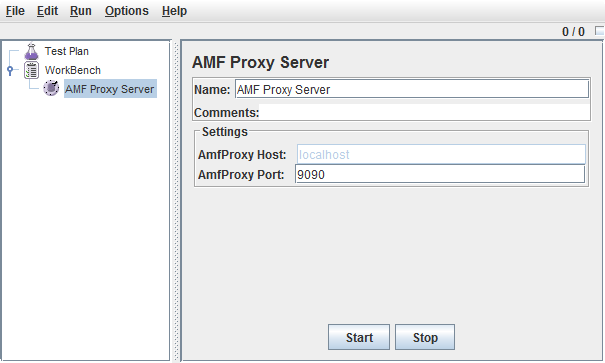
\includegraphics[height=60mm, width=80mm]{fig/development/proxySettings.png}}
\caption{Настройка прокси-сервера}
\label{ris:proxySettings.png}
\end{figure}

В поле AmfProxy Port необходимо указать номер порта, который будет слушать наш прокси сервер.
Если указать, например, 9090, то прокси-сервер будет запущен на localhost:9090.
Затем точно такие же настройки прокси-сервера устанавливаются в браузере, с помощью которого будет
производиться тестирование. Также стоит убедиться, что указанный Вами порт уже не занят другим приложением.

\subsection{Запись тестового сценария}

После того, как в AMF Proxy Server установлены все необходимые параметры, нажимается кнопка Start,
запускающая прокси-сервер.

\begin{figure}[h]
\center{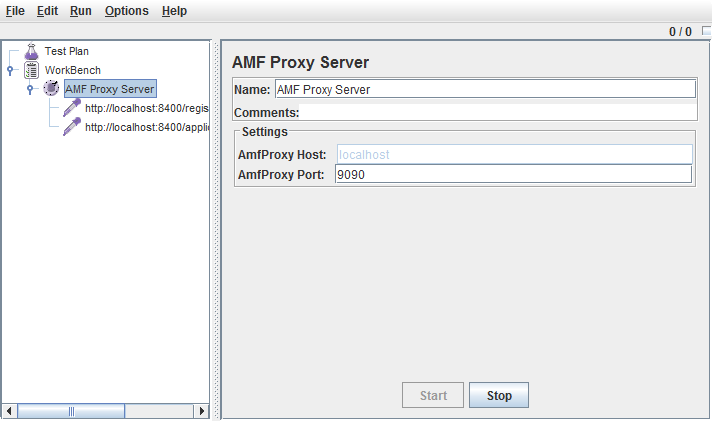
\includegraphics[height=60mm, width=80mm]{fig/development/proxyStart.png}}
\caption{Запуск прокси-сервера}
\label{ris:proxyStart.png}
\end{figure}

Затем тестируемое приложение открывается в браузере, для которого также
применены соответсвующие настройки прокси-сервера, и пользователь может выполнять с Flex приложением
необходимые операции, которые будут записываться AMF Proxy Server в виде элементов AMF RPC Sampler и в
дальнейшем могут быть перенесены в тест-план. Чтобы завершить запись тестовых запросов, необходимо
нажать кнопку Stop. После завершения записи тестов, все перехваченные запросы отображаются в дереве
элементов JMeter в качестве дочерних элементов AMF Proxy Server.

\subsection{Создание тест-плана}

Создание тест-плана в JMeter осуществляется следующим образом.
В первую очередь добавляется группа потоков - Thread Group (Test Plan > Threads (Users) > Thread Group).

\begin{figure}[h]
\center{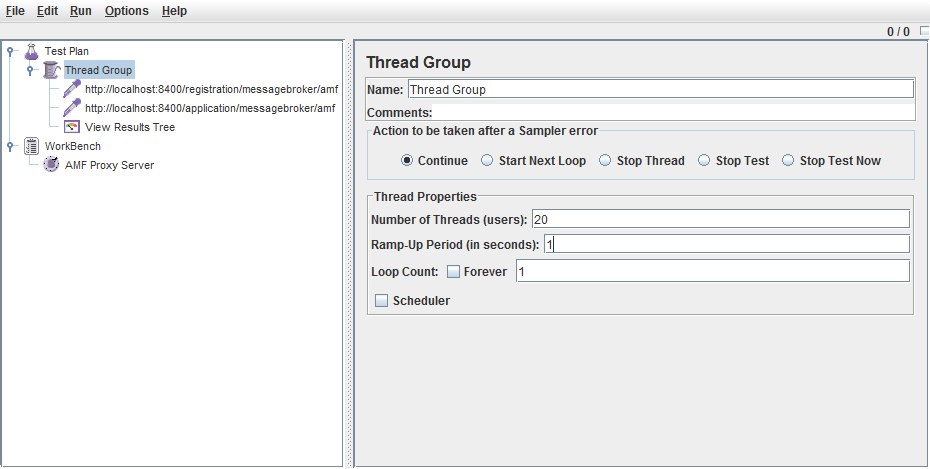
\includegraphics[height=60mm, width=80mm]{fig/development/testplan.png}}
\caption{Создание тест-плана}
\label{ris:testplan.png}
\end{figure}

Этот элемент является ключевым в тест-плане JMeter, именно его функционал отвечает за реализацию
нагрузочного тестирования --- многопоточного запуска последовательности тестовых шагов.
В данном элементе задается следующее:

\begin{enumerate}
\item Действия, которые будут производиться в случае, если в тест выполняется с ошибкой
(Action to be taken after a Sampler error);
\item Число потоков, в которое будут запускаться шаги тест-плана (Number of Threads);
\item Интервал, в течение которого будет запущено указанное в предыдущем параметре
число потоков (Ramp-Up Period);
\item Число повторений набора тестов (Loop Count);
\item Расписание запуска тестов (Scheduler).
\end{enumerate}

Затем в Thread Group в качестве дочерних элементов добавляются шаги тестов, которые
будут запускаться с указанными характеристиками. В нашем случае мы переносим элементы
AMF RPC Sampler, записанные с помощью прокси.
Помимо этого следует добавить визуалайзер результатов, чтобы иметь возможность
отслеживать ход тестового сценария (Thread Group > Add > Listener ).
JMeter предлагает большой выбор таких элементов, для примера будем использовать View Results Tree.
После того как план сформирован, он может быть сохранён. (File > Save Test Plan As...)

\subsection{Запуск тестов}

Чтобы запустить содержимое элемента Test Plan, необходимо выбрать в основном меню Run > Start.
После заврешения прогона тестов результаты их выполнения можно наблюдать в View Results Tree.

\section{Методика тестирования}



\end{document}